\documentclass[11pt, english]{article}
\usepackage[english]{babel}
\usepackage[utf8]{inputenc}



\usepackage{geometry}
 \geometry{
 a4paper,
 left=20mm,
 top=30mm,
 right=20mm
 }

\usepackage{wrapfig}
\usepackage{listings}
\usepackage{amsmath}
\usepackage{amsfonts}
\usepackage{amssymb}
\usepackage{amsthm} 
\usepackage{mathrsfs}
\usepackage{mathabx}
\usepackage{graphicx}
\usepackage{eurosym}
\usepackage{subfigure}
\usepackage{dsfont}
\usepackage{bbm}
\usepackage{tikz}
\usetikzlibrary{positioning,arrows.meta,calc}



\tikzset{
	arro/.style={
		->,
		>=latex
	},
	bloque/.style={
		draw,
		minimum height=1cm,
		minimum width=0.5cm
	}  
}



\newcommand{\su}[2]{\sum\limits_{#1}^{#2}}

\newcommand{\grafico}[5]{
\begin{figure}
[h!tbp]
\centering
\includegraphics[scale=#2, angle=#3]{#1}
%\captionsetup{width=13cm}
\caption{#4\label{#5}}
\end{figure}
}

\setlength{\parindent}{0pt}

\title{Open guide for Machine Learning: Theory}
\author{Roger Garriga Calleja \& Javier Mas Adell}
\date{\today}

\begin{document}
\maketitle

\section{Important probability's inequalities}

\subsection*{Markov's inequality}

If $X\geq 0$ is a non-negative random variable and $t>0$, then
\begin{equation}
	P(X\geq t)\leq \frac{\mathbb{E}X}{t}.
\end{equation}
\begin{proof}
	$X\geq t\mathbbm{1}_{X\geq t}$. Taking expectation on both sides: $\mathbb{E}X\geq \mathbb{E}t\mathbbm{1}_{X\geq t}=tP(X\geq t)$. \\ So, $P(X\geq t) \leq \frac{\mathbb{E}\mathbbm{1}_{X\geq t}}{t}$. \\ Q.E.D.
\end{proof}

\subsection*{Chebyshev's inequality}

For any random variable with finite variance
\begin{equation}
	P(|X-\mathbb{E}X|\geq t)\leq \frac{\text{Var} X}{t^2}.
\end{equation}

\begin{proof}
	$P(|X-\mathbb{E}X|\geq t)=P((X-\mathbb{E}X)^2\geq t^2)$. \\
	By Markov's inequality $P((X-\mathbb{E}X)^2\geq t^2)\leq \frac{(X-\mathbb{E}X)^2}{t^2}=\frac{\text{Var} X}{t^2}$.\\
	Q.E.D.
\end{proof}

In particular, if $S=\su{i=1}{n} X_i$ independent random variables, then $\text{Var}(S)=\sum\limits_{i=1}^n \text{Var}(X_i)$ and $=n\text{Var}(X_1)$ if they are independent identically distributed (iid from now on). So,
\begin{equation}
	P(|S-\mathbb{E} S|\geq t)\leq \frac{n\text{Var}(X_1)}{t^2}.
\end{equation}

That implies the weak law of large numbers, dividing by $n$:
\begin{equation}
	P(|\frac{1}{n}S-\mathbb{E}\frac{1}{n}S|\geq \epsilon) = P(|S -\mathbbm{E}S| \geq n\epsilon)\leq\frac{Var(S)}{(n\epsilon)^2} = \frac{Var(X_1)}{n\epsilon^2} \rightarrow 0\text{ as }n\rightarrow\infty.
\end{equation} 



\subsection*{Chernoff's bounds}

For any $\lambda>0$,
\begin{equation}
	P(X-\mathbb{E}X\geq t)\leq\frac{\mathbb{E}e^{\lambda(X-\mathbb{E}X)}}{e^{\lambda t}}.
\end{equation} 
\begin{proof}
	$P(X-\mathbb{E}X\geq t)=P(e^{\lambda(X-\mathbb{E}X)}\geq e^{\lambda t})$, now applying Markov's inequality $P(e^{\lambda(X-\mathbb{E}X)}\geq e^{\lambda t})\leq \frac{\mathbb{E}e^{\lambda(X-\mathbb{E}X)}}{e^{\lambda t}}$. \\ Q.E.D
\end{proof}

\subsection*{Hoeffding's inequality}

\textbf{Hoeffding's Lemma:} If $X$ is a random variable taking values in $[a,b]$, then $\mathbb{E}[e^{\lambda(X-\mathbb{E}X)}]\leq e^{\frac{\lambda^2(b-a)}{8}}$.
(In particular for $X\in[0,1]$, $\mathbb{E}[e^{\lambda(X-\mathbb{E}X)}]\leq e^{\frac{\lambda^2}{8}}$).\\

Though Hoeffding's Lemma and Chernoff's bounds, we get the Hoeffding's inequality:
\begin{equation}
	P(S-\mathbb{E}S\geq t)\leq e^{-\frac{2t^2}{n(b-a)^2}}.
\end{equation}

(In particular for $X\in[0,1]$, $P(S-\mathbb{E}S\geq t)\leq e^{-\frac{2t^2}{n}}$)

\begin{proof}
	Let $S = \sum_{i=1}^{n}X_i$ iid random variables. By Chernoff's bounds $P(S-\mathbb{E}S\geq t)\leq \underset{\lambda>0}{\text{min}}\frac{\prod\limits_{i=1}^n \mathbb{E}[e^{\lambda(X_i-\mathbb{E}X_i)}]}{e^{\lambda t}}$, now using Hoeffding's Lemma, $\underset{\lambda>0}{\min}\frac{\prod\limits_{i=1}^n \mathbb{E}[e^{\lambda(X_i-\mathbb{E}X_i)}]}{e^{\lambda t}}\leq \underset{\lambda>0}{\min}\frac{e^{(\lambda^2 n(b-a))/8}}{\lambda t}=\underset{\lambda>0}{\min}\ e^{\frac{\lambda^2n(b-a)}{8}-\lambda t}$. Minimizing (taking derivative to 0) we get $\lambda=\frac{4t}{n(b-a)}$, so $P(S-\mathbb{E}S\geq t)\leq e^{-\frac{2t^2}{n(b-a)^2}}$\\
	Q.E.D
\end{proof}

Normalizing we get $P(\frac{1}{\sqrt{n}}(S-\mathbb{E}S)\geq t)\leq e^{-\frac{2t^2}{(b-a)^2}}$.

\subsection*{Bernstein's inequality}

Let $X_1,\dots,X_n$ be independent such that $X_i\leq b$ for some $b > 0$ and let $v=\sum\limits_{i=1}^n\mathbb{E}[X_i^2]$. Then, $\forall t>0$,
\begin{equation}
	P(\sum\limits_{i=1}^n X_i - \mathbb{E}\sum\limits_{i=1}^n X_i \geq t)\leq e^{-\frac{t^2}{2(v+\frac{bt}{3})}}.
\end{equation}
If $X_i$ are iid with $\mathbb{E}X=0$, then $v=n\sigma^2$ ($\sigma^2=Var(X)$), so
\begin{equation}
	P(\sum\limits_{i=1}^n X_i\geq t)\leq e^{-\frac{t}{2n\sigma^2+\frac{2}{3}t}}.
\end{equation} 


\subsection{Jensen's inequality}

\subsection{Cauchy-Schwartz's inequality}

\section{Mean estimator}


The motivation of this section is to find a good estimator of the expected value of a population $X$ given a sample drawn from that population. That said, we assume that $X_1,\dots,X_n$ are independent identically distributed (iid from now on) random variables with expected value $\mathbb{E}X_1=m$. We would like to find a good empirical estimate $\hat{m}_n$ that is close to $m$. \\

Hence, the estimator will be a function $\hat{m}_n(x_1,\dots,x_n)$ of the observations we have that. A good estimator should have "small" error $|\hat{m}_n-m|$. However, since $\hat{m}_n$ is a random variable (it is a function of random variables) there are many ways to measure the error. In general it is measured as the expected value of a function $l:\Re\times\Re\rightarrow\Re_+$ called loss function, that symbolizes how much we "pay" by saying $m=\hat{m}_n$. Common examples of loss functions are $l(\hat{m}_n,m)=(\hat{m}_n-m)^2$ and $l(\hat{m}_n,m)=|\hat{m}_n-m|$. \\
A more flexible way of measuring the error is using the probability that $\hat{m}_n$ is at distance more than $\epsilon$, $P(|\hat{m}_n-m|>\epsilon)=\mathbb{E}\mathbbm{1}_{|\hat{m}_n-m|>\epsilon}$. This corresponds to the loss function $l(\hat{m}_n,m)=\mathbbm{1}_{|\hat{m}_n-m|>\epsilon}$.\\

The naive estimator is the sample mean $\hat{m}_n=\frac{1}{n}\sum\limits_{i=1}^n x_i$, which is unbiased and has a mean squared error (MSE) of $\mathbb{E}[(\hat{m}_n-m)^2]=\frac{\sigma^2}{n}$. But it behaves poorly in general if the variance is large. The probability of being far from the real mean can be bounded using the inequalities:
\begin{itemize}
	\item By Chebyshev's: $P(|\hat{m}_n-m|\geq \epsilon)\leq\frac{\sigma^2}{n\epsilon^2}$.
	\item By Hoeffding's: If $X_i\in [0,1]$, then $P(|\hat{m}_n-m|\geq \epsilon)\leq e^{-2n\epsilon^2}$.
	\item Applying Markov's in the sub-gaussian case ($\mathbb{E}e^{\lambda(X\mathbb{X})}\leq e^{\frac{\lambda^2\sigma^2}{2}}$) like we did in Hoeffding's lemma : $P(|\hat{m}_n-m|\geq \epsilon)\leq e^{-\frac{n\epsilon^2}{2\sigma^2}}$. 
\end{itemize}
In general it is difficult that we can apply Hoeffding's inequality or that we have a sub-gaussian distribution (in order to have $\mathbb{E}e^{\lambda X}=\int e^{\lambda x}f(x)\text{d}x<\infty$ we need the density $f(x)$ to beat $e^{\lambda x}$). So we should find an estimator of the mean more stable than the sample mean.

\subsection{Median of means estimator (MoM)}

The idea behind this estimator is to divide the data into $K$ blocks of size $l=\frac{n}{K}$ each, compute the mean in each block and compute the median of the means. \\

So, the $K$ blocks would be $\{x_1,\dots,x_l\},\{x_{l+1},\dots,x_{2l}\},\dots\{x_{(K-1)l+1},\dots,x_{Kl}\}$, the means $\mu_1=\frac{1}{l}\sum\limits_{i=1}^l x_i,\mu_2=\frac{1}{l}\sum\limits_{i=l+1}^{2l}x_1,\dots,\mu_K=\sum\limits_{i=(K-1)l+1}^{Kl}x_i$ and the estimator $\hat{m}_n=\text{median}(\mu_1,\dots,\mu_k)$.\\

Assuming that $Var(X)=\sigma^2<\infty$, by Chebyshev 
\begin{equation}
	|\mu_i-m|< \frac{2\sigma}{\sqrt{l}}\text{ with probability }\geq \frac{3}{4},
\end{equation}
for each $j=1,\dots,K$ (we could take a probability different of $\frac{3}{4}$ that may result in a better constant, but $\frac{3}{4}$ is good enough). 
\begin{proof}
	$P(|X-\mathbb{E}X|\geq\epsilon)\leq\frac{\sigma^2}{n\epsilon^2}=\delta\Leftrightarrow P(|X-\mathbb{E}X|<\frac{\sigma}{\sqrt{n\delta}}) \geq \frac{\sigma^2}{n\frac{\sigma}{\sqrt{n\delta}}} = 1-\delta$. Taking $\delta=\frac{1}{4}$, $\frac{\sigma}{\sqrt{n\delta}}=\frac{2\sigma}{\sqrt{n}}$.
\end{proof}
And for the estimator, $|\hat{m}_n-m|\geq \frac{2\sigma}{\sqrt{l}}$ iif at least half of the $\mu_1,\dots,\mu_K$ are $\frac{2\sigma}{\sqrt{l}}$ away from $m$. Then, the problem is reduced to the binomial and Hoeffding's inequality can be applied:
\begin{equation}
	P(\text{Bin}(K,\frac{1}{4})\geq \frac{K}{2})=P(\text{Bin}(K,\frac{1}{4})-\frac{K}{4}\geq \frac{K}{4})\leq e^{-\frac{2K^2}{16K}}=e^{-\frac{K}{8}}.
\end{equation} 
Then, we can choose $K$ according to the precision $\delta$ we want, $e^{-\frac{K}{8}}=\delta\Rightarrow K=[8\log\frac{1}{\delta})]$ so $l=\frac{n}{8\log\frac{1}{\delta}}$.\\

\textbf{Result:} MoM estimator with parameter $K=[8\log\frac{1}{\delta}]$ satisfies that $|\hat{m}_n-m|\leq 2\sigma\sqrt{\frac{8\log\frac{1}{\delta}}{n}}$. Notice that this inequality is sub-gaussian, 
\begin{equation}
	P(|\hat{m}_n-m|\geq\epsilon)\leq e^{-\frac{n\epsilon^2}{2\sigma^2}}=\delta\Leftrightarrow |\hat{m}_n-m|<\sigma\sqrt{\frac{2\log\frac{1}{\delta}}{n}}\text{ with probability }1-\delta,
\end{equation} 

This bound is much better than the one obtained by Chebyshev. However it has two downsides: MoM is not unbiased and the estimator depends on the precision $\delta$.


\section{Dimensionality Reduction}

\subsection{By Random Projection}
The idea is to map a set of $a_1,a_2,\dots,a_N$ points that belong to a space of dimension $D$, $\Re^D$ into a smaller space of dimension $d$, $\Re^d$ with $d<<D$. So we look for a function $f:\Re^D\rightarrow\Re^d$ such that $f(a_1),\dots,f(a_N)$ is a good representation of $a_1,\dots,a_N$. \\

In this case the fundamental characteristic of ``good representation" would be $||f(a_i) - f(a_j)|| \approx ||a_i - a_j||$ that the pairwise distances between points are preserved. This characteristic is important on clustering. But in general, if inside the set \{$a_1,\dots,a_N$\} there are $s$ points that are independent, then at most we can only reduce the dimension to $\Re^{s-1}$, which is not enough because we could have a number of points of the order of $N$, so the dimensionality reduction would be minimal.\\

However, if we allow some slack, the situation changes dramatically. We require that $f$ is such that

\begin{equation}
	1-\epsilon\leq\frac{||f(a_i)-f(a_j)||^2}{||a_i-a_j||^2}\leq 1+\epsilon, \text{ for some }\epsilon>0. 
\end{equation}

And it turns out that such an $f$ exists whenever $d\geq 8\frac{\log N}{\epsilon^2}$ (Johnson-Lindenstrauss lemma). That is, independently of D! Even more surprising is that to find such a function we only need to take $f$ to be linear, that is, $f(a) = Wa$, where $W=(W_{ij})$ is some random $d\times D$ matrix that projects the data points in $\Re^D$ to $\Re^d$.

We want to see that $||W(a_i-a_j)||^2\approx ||a_i-a_j||^2$. We will prove it for $W \sim \mathcal{N}(0, 1/d)$ and for any fixed $b\in \Re^D$, 
\begin{align}
	\mathbbm{E}||Wb||^2&= \mathbbm{E}\Bigg[\sum\limits_{i=1}^d\left(\sum\limits_{j=1}^D W_{ij}b_j\right)^2\Bigg]=\sum\limits_{i=1}^d\mathbbm{E}\Bigg[\left(\sum\limits_{j=1}^DW_{ij}b_j\right)^2\Bigg] \underset{\text{ind}}{=}\sum\limits_{i=1}^d\sum\limits_{j=1}^D\mathbbm{E}[W_{ij}^2bj^2]\\
	& \underset{b_j\text{ ctt}}{=}\sum\limits_{i=1}^d\sum\limits_{j=1}^Db_j\mathbbm{E}[W_{ij}^2]=\sum\limits_{i=1}^d\sum\limits_{j=1}^Db_j(\mathbbm{E}[W_{ij}^2] - \mathbbm{E}[W_{ij}]^2)\\
	&=\sum\limits_{i=1}^d\sum\limits_{j=1}^Db_jVar(W)=\frac{1}{d} \sum_{i=1}^d\sum\limits_{j=1}^Db_j^2=||b||^2.
\end{align}
In particular, $\mathbbm{E}||W(a_i-a_j)||^2=||(a_i-a_j)||^2$. Now we want it with high probability,
\begin{equation}
	\left\lvert\frac{||W(a_i-a_j)||^2}{||(a_i-a_j)||^2}-1\right\lvert<\epsilon.
\end{equation}
We will denote $c_{ij}=\frac{(a_i-a_j)}{||a_i-a_j||}$. Note that, by definition $||\frac{x}{||x||}|| = \frac{1}{||x||}||x|| = 1$, hence $c_{ij}$ is the unit vector.
	
Then, $\| W c\|^2-1=\su{i=1}{d}\left(\su{j=1}{D}W_{ij}c_j\right)^2-1$. Note that $\su{j=1}{D}W_{ij}c_j = N_i \sim \mathcal{N}(0,\frac{1}{d})$. Furthermore, $\su{i=1}{d}\mathbb{E}[N_i^2]=1$. Putting both things together, we can write 
\begin{equation}
	\|Wc\|^2-1=\sum\limits_{i=1}^d\left(N_i^2-\mathbb{E}[N_i^2]\right).
\end{equation} 

Now, note that $Z = \sum_{i=1}^{d}N_i^2 \sim \mathcal{X}^2(d)$ is a sum of squared normal random variables, hence we can apply Chernoff bounds
$P(|\|Wc_{ij}\|-1>\epsilon)\leq e^{-\frac{\epsilon^2d}{4}}$, which implies
\begin{equation}
	P(\underset{i,j=1,\dots N}{\max}\|Wc_{ij}\|^2-1>\epsilon)\leq \left(\begin{array}{c}
	N\\
	2
	\end{array}\right)e^{-\frac{\epsilon^2d}{4}}\leq \frac{N^2}{2}e^{-\frac{\epsilon^2d}{4}}.
\end{equation}
If we want the probability to be less than $\delta$, then we find that $d\geq \frac{4}{\epsilon^2}\log\frac{N^2}{2\delta}$\\
 
\textbf{Johnson-Lindestrauss lemma:}
Given $a_1,\dots,a_n$, there exists $f:\Re^D\rightarrow\Re^d$ such that for all $i,j=1,\dots,N$, 
\begin{equation}
	1-\epsilon\leq\frac{\| f(a_i)-f(a_j)\|^2}{\|a_i-a_j\|^2}\leq 1+\epsilon.
\end{equation}
whenever $d\geq \frac{8}{\epsilon^2}\log N$.\\

Especial remarks after this result is that the best dimension we can hope for (even allowing $f$ to be non-linear) is $d\sim\frac{\log n}{\epsilon^2}$. That no deterministic construction is known. And that Euclidian distance is crucial in dimensionality reduction.


\section{Basic decision theory}

The idea is to predict the value of a random variable $Y\in T$ assuming that we know the distribution of $Y$. The set $ T$ may be $\{0,1\},\{1,\dots,N\},\Re,\Re^d,\dots$. We will note our prediction as $p\in T$. The quality of the predictor is measured by a loss function
$$l: T\times T\rightarrow\Re_{+}.$$

There are many functions that can be used as loss functions. For $ T=\{0,1\}$ a natural one is $l(y,p)=\mathbbm{1}_{y\neq p}$. An asymmetric version that penalize more one error than the other would be
$$l(y,p)=\left\{\begin{array}{ll}
a & \text{if } y=0,p=1\\
b & \text{if } y=1,p=0\\
0 & \text{otherwise}
\end{array}\right.$$
For $ T=\Re^d$ we may have 
$$l(y,p)=\|y-p\|^2,$$
$$l(y,p)=\|y-p\|.$$

We will focus on the \textit{risk} of the decision $p$. Which is
\begin{equation}
	R(p)=\mathbb{E}l(y,p).
\end{equation}
For the risk function, the optimal prediction would be $p^*\in T$ such that $p^*=\underset{p\in T}{\text{argmin}}R(p)$. Then, the optimal risk is noted $R^*=R(p^*)$.\\

For example, if $ T=\{0,1\}$ and $l(y,p)=\mathbbm{1}_{y\neq p}$, the risk would be 
\begin{equation}
	R(p)=\mathbb{E}l(Y,p)=p(Y=0)\mathbbm{1}_{p=1}+p(Y=1)\mathbbm{1}_{p=0}.
\end{equation}
Then, $R^*=R(p^*)=\min(p(Y=0),p(Y=1))$.\\

For $ T=\Re$ and $l(y,p)=(y-p)^2$, the risk would be $R(p)=\mathbb{E}(Y-p)^2=\mathbb{E}[Y^2]-2p\mathbb{E}[Y]+p^2$. The minimizer would be $p^*=\mathbb{E}Y$. If the loss function was $l(y,p)=|y-p|$, $p^*$ would be the median of $Y$. That is also a way to define the median for higher dimensional spaces $Med(Y)=\underset{p}{\text{argmin}}\|Y-p\|^2$.

\subsection{Prediction problem with a covariate}

Let ($X,Y$) be a pair of random variables taking values in $\Omega\times T$. We usually call $X$ observations, features or covariates and $Y$ label or target. We want to predict $Y$ given an observed value $X$. If we assume that the joint distribution of ($X,Y$) is known, a predictor $p$ is a function of $X$ $p:\Omega\times T$. Given a loss function $l:T\times T\rightarrow \Re_{+}$, the loss function will be $l(p(X),Y)$ and the risk $R(p)=\mathbb{E}l(p(X,Y))$. Then, the risk can also be written as 
\begin{equation}
	R(p)=\mathbb{E}[l(p(x),Y)]=\mathbb{E}_X\mathbb{E}_{Y|X}[l(p(X),Y)|X].
\end{equation}


\textbf{Example\\}
Binary classification: $T=\{0,1\}$, $l(p,Y)=\mathbbm{1}_{p\neq Y}$. Then the risk function would be $R(p)=\mathbb{E}\mathbbm{1}_{p(X)\neq Y}=P(p(X\neq Y))=\mathbb{E}\mathbb{P}(p(X)\neq Y|X)$. So $p$ would be minimized as $p^*=\left\{\begin{array}{ll}
1 & \text{if }\mathbb{P}(Y=1|X)>\frac{1}{2}\\
0 & \text{otherwise}
\end{array}\right.$. This $p(Y=1|X)$ is called a posteriori probability (sometimes noted by $\eta(X)$). Then, the optimal risk would be $\mathbb{E}[\min(\eta(X),1-\eta(X))]$. 

Basically the risk minimization and optimal predictor with a covariate work as without it but instead of marginal probabilities we take conditional probabilities $Y|X$.\\

\textbf{Notation in binary classification:\\}
A posteriori probability: $\eta(x)=\mathbb{P}(Y=1|X=x)=\mathbb{E}(Y|X=x)$.\\
A priori probabilities: $q_0=\mathbb{P}(Y=0)$, $q_1=\mathbb{P}(Y=1)$.\\
Marginal distribution of $X$: $\mu(A)=\mathbb{P}(X\in A)$.\\
Conditional densities for $X$ given $Y$: $f_0(X)=f(X|Y=0)$, $f_1=(X|Y=1)$.\\

\textbf{Example\\}

Let $f_0(x)=\frac{1}{\sqrt{2\pi}}e^{-\frac{x^2}{2}}\sim N(0,1)$, $f_1(x)=\frac{1}{\sqrt{2\pi}}e^{-\frac{(x-1)^2}{2}}$, $q_0=\frac{1}{2}$, $q_1=\frac{1}{2}$. Then the a posteriori probabilities would be
$$\mathbb{P}(Y=1|X=x)=\frac{f_1(x)q_1}{f_1(x)q_1+f_0(x)q_0},$$
$$\mathbb{P}(Y=0|X=x)=\frac{f_0(x)q_0}{f_1(x)q_1+f_0(x)q_0}.$$
Then, $p^*(x)=\left\{\begin{array}{ll}
1 & \text{if }\frac{f_1(x)}{f_0(x)}>\frac{q_0}{q_1}\\
0 & \text{otherwise}
\end{array}\right.$. If $q_0=q_1=\frac{1}{2}$ we choose the $i$ with $f_i(x)$ higher, otherwise it would depend on how different are the marginals.\\

The problem is that in general we do not know the conditional distribution $X|Y$, we have data instead $D_n=\{(X_1,Y_1),\dots,(X_n,Y_n)\}$. Our assumption will be that the $(X_i,Y_i)$ are iid. With that, we will try to predict the next $Y_{n+1}$ given a new observation $X_{n+1}$. So, the predictor will depend on the new observation and the data $p(X_{n+1},D_n)=p_n(X_{n+1})$. The goal is to find a predictor $p_n$ such that the risk $R(p_n)=\mathbb{E}[l(p_n(X_{n+1}),Y)|D_n]$ is as close to $R^*$ as possible. \\
We will measure how far is the predictor's risk $R^* = \mathbb{P}(R(p_n)-R^*>\epsilon)$ and minimize it for all distributions.\\

We define a prediction rule to be \textbf{consistent} if $$\mathbb{E}R(p_n)\underset{n\rightarrow\infty}{\longrightarrow} R^*\Leftrightarrow \mathbb{P}(R(p_n)-R^*>0)\rightarrow 0\text{ }\forall \epsilon>0.$$

\textbf{No-free-lunch theorem:} For all prediction rules $p_n$ and every sample size $n$, no matter how big $n$ is, there exist a distribution of $X,Y$ such that $\mathbb{E}R(p_n)-R^*>0.49$ (for classification, but in general is the same, there always exist a distribution that makes the prediction perform bad). \\

In order to remedy this, we restrict the class of distributions we target or the class of prediction rules. So $R^*$ will be the minimum in the class. The next step is to estimate the risk using a good estimator $\hat{R}_n(p_n)$ of $R(p_n)$. This estimate should be such that $|R(p_n)-\hat{R}_n(p_n)|$ is small for all distribution given a sample of size $n$. At least $R(p_n)\leq \hat{R}(p_n)$ and small with high probability.
\subsection{Classification}

First suppose that our data is $D_n=(Y_1,\dots,Y_n)$, $Y_i\in\{0,1\}$ (no covariates $X$).\\

As a first approach we could consider $p_n=Y_1$, $R(p_n)=\mathbbm{1}_{Y_1=0}\mathbb{P}(Y=1)+\mathbbm{1}_{Y=1}\mathbb{P}(Y=0)$. However, as $R^*=\min\{\mathbb{P}(Y=0),\mathbb{P}(Y=0)\}$, the expected value will not be consistent $R^*\leq\mathbb{E}R(p_n)=2\mathbb{P}(Y=0)\mathbb{P}(Y=1)\leq 2R^*$.\\

A better idea is to pick $p_n$ as the majority rate, meaning $p_n=\left\{\begin{array}{ll}
0 & \text{if }\frac{1}{n}\sum\limits_{i=1}^nY_i<\frac{1}{2}\\
1 & \text{otherwise}
\end{array}\right.$. For $n$ big that would tend to $p^*=\left\{\begin{array}{ll}
1 & \text{if }\mathbb{P}(Y=1|X)>\frac{1}{2}\\
0 & \text{otherwise}\end{array}\right.$. \\
This predictor is consistent: $R(p_n)=\eta\mathbbm{1}_{\sum\limits_{i=1}^nY_i<\frac{n}{2}}+(1-\eta)\mathbbm{1}_{\sum\limits_{i=1}^nY_i>\frac{n}{2}}$. The expected value  of the risk would be
\begin{equation}
	\mathbb{E}R(p_n)=\eta\mathbb{P}(\text{Bin}(n,\eta)<\frac{n}{2})+(1-\eta)\mathbb{P}(\text{Bin}(n,\eta)\geq\frac{n}{2}).
\end{equation}
Using that $\mathbb{P}(\text{Bin}(n,\eta)\geq\frac{n}{2})=1-\mathbb{P}(\text{Bin}(n,\eta)<\frac{n}{2})$ and assuming without lost of generality $\eta<\frac{1}{2}$ we get $\mathbb{E}R(p_n)=\eta+(1-2\eta)\mathbb{P}(\text{Bin}(n,\eta)\geq\frac{n}{2})$. Since in this case $R^*=\eta$, using Hoeffding's inequality we get that 
\begin{equation}
	\mathbb{E}R(p_n)-R^*=\eta+(1-2\eta)\mathbb{P}(\text{Bin}(n,\eta)\geq\frac{n}{2})\leq e^{-2n(\frac{1}{2}-\eta)^2},
\end{equation}
which decreases fast with $n$. The maximum will be taken for $\eta\approx \frac{1}{2}-\frac{1}{\sqrt{n}}$.

Now let's consider a more realistic situation in which we have also covariates. Our data would be $D_n=(X_1,Y_1),\dots,(X_n,Y_n)$, where $(X_n,Y_n)\in\Omega\times\{0,1\}$. In this framework the goal is to predict $Y_{n+1}$ once we have observed $X_n$. The optimal decision would be 
\begin{equation}
	p^*(X)=\left\{\begin{array}{ll}
	1 & \text{if }\eta(X)\geq\frac{1}{2}\\
	0 & \text{otherwise} 
	\end{array}\right.,
\end{equation}
known as Bayes decision (even though Bayesian Statistics is not involved) (recall $\eta(x)=\mathbb{P}(Y=1|X=x)$. Then, the optimal risk (called Bayes risk) would be 
\begin{equation}
	R^*=\mathbb{E}\min\{\eta(X),1-\eta(X)\}.
\end{equation}

\subsubsection{The nearest neighbor rule}

With this rule, we predict the new observation as the same category as his nearest neighbor. We would order the data as $(X_{(1)}(x),Y_{(1)}(x),\dots,(X_{(n)}(x),Y_{(n)}(x)$ according to the distance to $X$. That is $d(X_{(1)}(x),x)\leq\dots\leq d(X_{(n)}(x),x)$. The first question is how to define the notion of distance in each problem. We could use $d(x,y)=\|x-y\|_1,\dots,d(x,y)=\|x-y\|_{\infty}$, or also in general $d(x,y)=\sqrt{(x-y)^TA(x-y)}$, where $A$ is a symmetric positive semidefinite matrix.\\

However, when we increase the dimension we suffer the \textbf{curse of dimensionality}, the probability of being near decays exponentially with the dimensions. Suppose that our $X$ are uniformly distributed in $[0,1]$, then
\begin{equation}
	\mathbb{P}(d(x,X_{(1)}(x))>\epsilon)=\mathbb{P}(d(x,X_1)>\epsilon),\dots,\mathbb{P}(d(x,X_n)>\epsilon)=\mathbb{P}(d(x,X_1)>\epsilon)^n=(1-\mathbb{P}(d(x,X_1)\leq \epsilon)).
\end{equation}
As $X$ are iid uniform distributions, $\mathbb{P}(d(x,X_1)\leq \epsilon)=\epsilon^dv_d$, where $v_d$ is the volume of the unit ball in $\Re^d$. So
\begin{equation}
	\mathbb{P}(d(x,X_{(1)}(x))>\epsilon)=(1-v_d\epsilon^d)^n\leq e^{-v_dn\epsilon^d},
\end{equation}
(using $1-x\approx e^{-x}$ for $x$ small). That will be small if $n\epsilon^d$ is huge, meaning that $\epsilon\geq \sqrt[d]{n}$. That means that for $d=1$, $d(x,X_{(1)}(x))$ is of the order $\frac{1}{n}<\frac{1}{100}\Leftrightarrow n\geq 100$; for $d=2$, $\frac{1}{n}<\frac{1}{100}\Leftrightarrow n\geq 10000$; for $d=10$, $\frac{1}{n}<\frac{1}{100}\Leftrightarrow n\geq 100^{10}$. So the distance between points increases very fast with the dimension. However, $\forall d$, $d(x,X_{(1)}(x))\rightarrow 0$ in probability when $n\rightarrow\infty$. This is true for all distributions.\\

Remark: Nearest neighbor works if the classes are well separated. Then, even if the distance is big, it is still much smaller than the distance to the nearest of the other class. This tells us that in order to increase dimensionality (adding new variables) we better do it with variables that give us real information. Adding unimportant information adds noise that difficult classification.\\

\textbf{Theorem:} The expected risk of the nearest neighbor rule is 
\begin{equation}
	\underset{n\rightarrow \infty}{\lim}\mathbb{E}R(p_n^{NN})=2\mathbb{E}[\eta(x)(1-\eta(x))]=R_{NN}.
\end{equation}
That is true for all distributions.\\

As $\min(\eta,1-\eta)\leq2\eta(1-\eta)\leq 2\min(\eta,1-\eta)$, we always have that $R^*\leq R_{NN}\leq 2R^*(1-R^*)$, so $R_{NN}$ will only be consistent whenever $R^*=0$. That means that it will only be consistent if we $Y$ is a deterministic function of $X$.\\

\subsubsection{K-nearest neighbor rule}

The K-NN rule takes a majority vote among the $K$ closest points to predict. This rule have the same property as the previous one, $d(X_{(k)}(x),x)\underset{\scriptsize{n\rightarrow \infty}}{\longrightarrow}0$. \\

The risk for a general $K$ would be $R^{K-NN}=P(Y\neq \text{majority}\{Y_{(1)},\dots,Y_{(K)}\})$. For $K=3$ this will happen if $Y=1$ and the at least two of the nearest neighbors are 0, that is if either two of them are 0 or the three are 0 (similarly for $Y=0$). So, $P(Y\neq \text{majority}\{Y_{(1)},Y_{(3)},Y_{(3)}\})=\eta[(1-\eta)^3+3\eta(1-\eta)^2]+(1-\eta)[\eta^3+3(1-\eta)\eta^2]$ working out the equations we get $P(Y\neq \text{majority}\{Y_{(1)},Y_{(3)},Y_{(3)}\})=\eta(1-\eta)+4\eta^2(1-\eta)^2$. Then, the risk of the 3 nearest neighbor will be
\begin{equation}
	R^{3-NN}=\mathbb{E}[\eta(x) (1-\eta(x))]+4\mathbb{E}[\eta(x)^2(1-\eta(x))^2]\leq2\mathbb{E}[\eta(x)(1-\eta(x))]=R^{NN}
\end{equation}
If we develop in general for any $K$, we get
\begin{align}
	R^{K-NN} = &\mathbb{E}[\eta(X)\mathbb{P}\left(\text{Bin}(K,\eta(X))<\frac{K}{2}|X\right)+(1-\eta)\mathbb{P}\left(\text{Bin}(K,\eta(X))>\frac{K}{2}|X\right)]=\\
	= & \mathbb{E}[\min(\eta(X),1-\eta(X))]+\mathbb{E}[(2\eta(X)-1)\mathbb{P}\left(\text{Bin}(K,\min(\eta,\eta-1))>\frac{K}{2}|X\right)]\leq\\
	\underset{\scriptsize{\text{Hoeffding}}}{\leq} & R^*+e^{-2K|\eta(X)-\frac{1}{2}|^2}\leq R^*+\underset{\eta}{\max}|2\eta-1|e^{-2K|\eta(X)-\frac{1}{2}|^2}\leq\\
	\leq & R^*+\frac{1}{\sqrt{eK}},
\end{align}
where the last inequality comes by maximizing the expression. This bound decreases with the number of neighbors we take, if $K$ goes to infinity in a way that $\frac{K}{n}$ goes to 0 (for example $K=\sqrt{n}$ or $K=\log n$) then the risk converges to $R^*$ for all distributions. So, it would be universally consistent. \\

Nearest neighbor rules are examples of averaging rules, the simplest such rules are partitioning classifiers. These are rules that partition the space into small cubes and take a majority vote within the cell of the partition where the point $X$ to be classified lies. If $h$ is the size of the cube, and $h\rightarrow 0$ such that $nh^d\rightarrow \infty$ for $n\rightarrow\infty$, then the rule is universally consistent. 
Although the problem becomes dangerous when we increase the dimensions, because when one divides the space in cells of length $h$ the number of cells increases exponentially with the dimension. That makes the space full of cells and, as in order to be able to average inside each cell we need a fair number of points on it, we would need a lot of points to populate all the cells. We suffer the curse of dimensionality.\\

\section{Empirical risk minimization}

Let $g:\Omega\rightarrow\{0,1\}$ be a classifier that not depends on data. Given data $D_n=(X_1,Y_1),\dots,(X_n,Y_n)$, to know how good the estimator is we can estimate the risk as $R(g)=\mathbb{P}(g(X)\neq Y)$ by $R_n(g)=\frac{1}{n}\sum\limits_{i=1}^n\mathbbm{1}_{g(X_i)\neq Y_i}$. By Hoeffding's inequality we know that with probability $\geq 1-\delta$, 
\begin{equation}
	|R_n(g)-R(g)|\leq\sqrt{\frac{\log\frac{2}{\delta}}{2n}}.
\end{equation}
Now, the idea would be to know among different classifiers which is the best. That is given $N$ classifiers $g_1,\dots,g_N: X\rightarrow\{0,1\}$, choose the one that has less risk. We can estimate the risk with the same data and pick the best one, but this does not mean that in general it will be the best classifier.\\

We can estimate the risk of each classifier $g_j$ as $R_n(g_j)=\frac{1}{n}\sum\limits_{i=1}^n \mathbbm{1}_{g_j(X_i)\neq Y_i}$. For each classifier we have the above inequality, but the risks are not independent of the classifier rule used. We will use the union bound ($\mathbb{P}(\bigcup\limits_{i=1}^n A_i)\leq\sum\limits_{i=1}^n\mathbb{P}(A_i)$).
\begin{align}
	\mathbb{P}(\underset{j=1,\dots,N}{\max}|R_n(g_j)-R(g_j)|\geq\epsilon)=\mathbb{P}(\bigcup\limits_{j=1}^n\{|R_n(g_j)-R(g_j)|\geq \epsilon\})\\
	\leq\sum\limits_{j=1}^n\mathbb{P}(|R_n(g_j)-R(g_j)|\geq\epsilon)\leq 2Ne^{-2n\epsilon^2}=\delta.
\end{align}
Now, solving for $\delta$ we get that with probability $\geq 1-\delta$, \begin{equation}
	|R_n(g_j)-R(g_j)|\leq\sqrt{\frac{\log\frac{2 N}{\delta}}{2n}}.
\end{equation}

One important consequence of this is that if we take a classifier rule depending on data $D_n$ $\hat{p}_n:\Omega\times(\Omega\times\{0,1\})^n\rightarrow \{0,1\}$ that picks a classifier from the set $\{g_1,\dots,g_N\}$. And we estimate the risk of $\hat{p}_n$ by $R_n(\hat{p}_n)= \frac{1}{n}\mathbbm{1}_{\hat{p}_n(X_i)\neq Y_i}$, then with probability $\geq 1-\delta$
\begin{equation}
	|R_n(\hat{p}_n-R(\hat{p}_n))|\leq \sqrt{\frac{\log\frac{2N}{\delta}}{2n}}.
	\label{riskbound}
\end{equation}
Which implies that we can bound the theoretical risk of $\hat{p}_n$ from data as $R(\hat{p}_n)\leq R_n(\hat{p}_n)+ \sqrt{\frac{\log\frac{2N}{\delta}}{2n}}$ (with probability $\geq 1-\delta$). We still have the bound depending on the number of classifiers in the class, which can be huge.\\

Now, we will denote $\hat{p}_n=\underset{g_1,\dots,g_N}{\text{argmin}}R_n(g_j)$ the chosen classifier that empirically minimizes the risk and $\bar{p}=\underset{g_1,\dots,g_N}{\text{argmin}}R(g_j)$ the best classifier (that minimizes the theoretical risk). Let's see how close they are regarding their risk bounding the excess of risk:
\begin{equation}
	R(\hat{p}_n)-R(\bar{p})=(R(\hat{p}_n)-R_n(\hat{p}_n))+(R_n(\hat{p}_n)-R(\bar{p}_n)).
\end{equation}
Observe that $R(\hat{p}_n)-R_n(\hat{p}_n)\leq\underset{j=1,\dots,N}{\max}R(g_j)-R_n(g_j)$ ($\hat{p}_n$ is one of the $g_j$), also $R_n(\hat{p}_n)\leq R_n(\bar{p}_n)$ ($\hat{p}_n$ is chosen minimizing the empirical risk and $\bar{p}_n$ is the theoretical minimum) $\Rightarrow R_n(\hat{p}_n)-R(\bar{p}_n)\leq \underset{j=1,\dots,N}{\max}R_n(g_j)-R(g_j)$. Using (\ref{riskbound}) we can bound the excess risk by $R(\hat{p}_n)-R(\bar{p})\leq \sqrt{\frac{2\log\frac{2N}{\delta}}{n}}$ with probability $\geq 1-\delta$. This bound is very conservative, working a bit more we can get to
\begin{equation}
	R(\hat{p}_n)-R(\bar{p})\leq c\left(\sqrt{\frac{R(\bar{p})\log\frac{N}{\delta}}{n}}+\frac{\log\frac{N}{\delta}}{n}\right), \text{ }c \text{ constant}.
\end{equation}
\subsection{The resubstitution estimate:}

Let $p_n$ be a data-based estimate trained on $D_n=(X_1,Y_1),\dots,(X_n,Y_n)$. We want to estimate the risk $R(p_n)=\mathbb{P}(p_n(X)\neq Y|D_n)$ based on the same data $D_n$. The resubstitution estimate is just counting how many errors we did on our data
\begin{equation}
	R_n(p_n)=\frac{1}{n}\sum\limits_{i=1}^n\mathbbm{1}_{p_n(x_i)\neq Y_i}.
\end{equation}
Observe that in this case this is not a sum of independent variables, because $p_n$ depends on $X_i$. However, if $p_n$ is given by a fixed class $\mathcal{C}$ of non-data-dependent classifiers, then 
\begin{equation}
	|R_n(p_n)-R(p_n)|\leq\underset{g\in\mathcal{C}}{\max}|R_n(g)-R(g)|.
\end{equation}
If the classifier chooses from a small class, then the resubstitution estimate would work because we could bound it, otherwise it would be impossible. Observe that in particular the 1-NN has $R_n(p_n)=0$ (for each point the nearest neighbor will be itself).

\subsection{The deleted (or leave one out crossvalidation) estimate}

In this case the empirical risk would be computed as the sum of errors made on each point, but for every point $i$ we would train a $p_n^{(i)}$ with the data except $i$, so $p_n^{(i)}$ would be train on $D_n^{(-i)}=(X_1,Y_1),\dots,(X_{i-1},Y_{i-1}), (X_{i+1},Y_{i+1}),\dots,(X_n,Y_n)$.
\begin{equation}
	R_n^{(D)}(p_n)=\frac{1}{n}\sum\limits_{i=1}^n\mathbbm{1}
_{p_n^{(i)(X_i)\neq Y_i}}.
\end{equation}
Now, we don't have the dependence problem, $p_n^(i)$ does not depend on $(X_i,Y_i)$. And
\begin{equation}
	\mathbb{P}(p_n^{(i)}(X_i)\neq Y_i|D_n^(-i))=R(p_n^(i)),
\end{equation}
Taking expectation over the $X_i$ we get
\begin{equation}
	\mathbb{E}R_(p_n^{(i)})=\mathbb{E}R(p_n^(j)),\text{ for any }j=1,\dots,n.
\end{equation}
In particular 
\begin{equation}
	\mathbb{E}R_(p_n^{(i)})=\mathbb{E}R(p_n^(n))=\mathbb{E}R(p_{n-1}).
\end{equation}
So, the expected value is almost unbiased, 
\begin{equation}
	\mathbb{E}R_n^(D)(p_n)=\mathbb{E}R(p_{n-1}).
\end{equation}

In general saying something about $\mathbb{P}(|R_n^{(D)}-R(p_n)|>t|)$ is a challenge. All the dependencies that are when leaving one out are not trivial, so a lot of different classes have been studied to see in their particular case how it behaves. In practice we use the approximation that it is the same more or less when leaving one out, which works fairly well if we have a lot of data.

\subsection{Data splitting}

Suppose we have $N$ data-dependent classifiers $p_n^{(1)},\dots,p_n^{(N)}$ trained on the same data $D_n=(X_1,Y_1),\dots,(X_n,Y_n)$. And suppose we have $m$ additional data points $D_m'=(X_1',Y_1'),\dots,(X_m',Y_m')$ to test the performance. Then, we may define \begin{equation}
	R_n'(p_n^{(j)})=\frac{1}{m}\sum\limits_{i=1}^m\mathbbm{1}_{p_n^{(j)}(X_i')\neq Y_i'}.
\end{equation}
Now the classifiers do not depend on the test data, $R_m'(p_n^{(j)})$ will depend on $D_n$ and $D_m'$, and $R(p_n^{(j)})$ will depend only on $D_n$.
\begin{equation}
	|R_m'(p_n^{(j)}-R(p_n^{(j)})|\leq \underset{j=1,\dots,N}{\max}|R_m'(p_n^{(j)})-R(p_n^{(j)})|.
\end{equation}
If we condition now on $D_n$, then $p_n^{(j)}$ will be a fixed classifier not dependent on data, so we can bound it as
\begin{equation}
	|R_m'(p_n^{(j)}-R(p_n^{(j)})|\leq \sqrt{\frac{\log\frac{2N}{\delta}}{2m}},
\end{equation}
with probability $\geq 1-\delta$ respect to $D_m'$ conditioned on $D_n$. \\

\subsection{Vapnik–Chervonenkis (VC) theory}

We will try to quantify overfitting by taking into account the structure of the class of classifiers. Given a class $\mathcal{C}$ of non-data-dependent classifiers, we want to understand 
\begin{equation}
	\underset{g\in\mathcal{C}}{\max}|R_n(g)-R(g)|,
\end{equation}
where $R_n(g)=\frac{1}{n}\sum\limits_{i=1}^n\mathbbm{1}_{g(X_i\neq Y_i)}$ and $R(g)=\mathbb{P}(g(X)\neq Y)$. We know that if $\hat{g}_n=\underset{g\in\mathcal{C}}{\text{argmin}}R_n(g)$, then $R(\hat{g}_n)-\underset{g\in\mathcal{C}}{\min}R(g)\leq2\underset{g\in\mathcal{C}}{\min}|R_n(g)-R(g)|$.\\

Also, we have seen that if $\mathcal{C}$ is finite, then with probability $\geq 1-\delta$ the maximum is $\leq \sqrt{\frac{\log\frac{2N}{\delta}}{2n}}$. Observe that $R_n(g)$ counts for each $g$ how many mistakes it takes, so it is a binomial random variable $R_n(g)\sim \frac{1}{n}Bin(n,R(g))$. So, we are looking for the deviation of binomials with their expected value.\\

Let's start simplifying the notation. Let $X_1,\dots,X_n$ be iid taking values on $\Omega$. For $A\subset \Omega$, we define $P(A)=P(X\in A)$ and $P_n(A)=\frac{1}{n}\sum\limits_{i=1}^n\mathbbm{1}_{X_i\in A}$. And let $\mathcal{A}$ be a class of sets $A$. We are interested in 
\begin{equation}
	\underset{A\in\mathcal{A}}{\max}|P_n(A)-P(A)|.
\end{equation}
This notation is more general, the case of study is when $(X_i,Y_i)\rightarrow X_i$ ($\mathcal{C}\rightarrow \mathcal{A}$). For the finite case, $\mathcal{A}=\{A_1,\dots,A_N\}$, with probability $\geq 1-\delta$ we got that 
\begin{equation}
	\underset{A\in\mathcal{A}}{\max}|\mathbb{P}_n(A)-\mathbb{P}(A)|\leq\sqrt{\frac{\log\frac{2N}{\delta}}{2n}}.
\end{equation}
Let us bound now the expected value $\mathbb{E}\underset{A\in\mathcal{A}}{\max}(\mathbb{P}_n(A)-\mathbb{P}(A))$, to do so let's first take the exponential for $\lambda>0$
\begin{align}
	e^{\lambda\mathbb{E}\text{ }\underset{A\in\mathcal{A}}{\max}(\mathbb{P}_n(A)-\mathbb{P}(A))}\underset{\text{Jensen's}}{\leq}\mathbb{E}e^{\lambda\text{ }\underset{A\in\mathcal{A}}{\max}(\mathbb{P}_n(A)-\mathbb{P}(A))}.
\end{align}
As the exponential function is increasingly monotonous, the maximum value of the exponent leads to the maximum value of the exponential, so 
\begin{align}
	&\mathbb{E}e^{\lambda\text{ }\underset{A\in\mathcal{A}}{\max}(\mathbb{P}_n(A)-\mathbb{P}(A))}=\mathbb{E}\text{ }\underset{A\in\mathcal{A}}{\max}\text{ }e^{\lambda(\mathbb{P}_n(A)-\mathbb{P}(A))}\leq\mathbb{E}\sum\limits_{A\in\mathcal{A}}e^{\lambda(\mathbb{P}_n(A)-\mathbb{P}(A))}=\\
	&\sum\limits_{A\in\mathcal{A}}\mathbb{E}e^{\lambda(\mathbb{P}_n(A)-\mathbb{P}(A)}\underset{\text{Hoeffding's}}{\leq}\sum\limits_{A\in\mathcal{A}}e^{\frac{\lambda^2}{8n}}=Ne^{\frac{\lambda^2}{8n}}.
\end{align}
Now, applying logarithm on the beginning and on the end of the inequality, we get
\begin{equation}
	\mathbb{E}\underset{A\in\mathcal{A}}{\max}(\mathbb{P}_n(A)-\mathbb{P}(A))\leq\frac{\log N}{\lambda}+\frac{\lambda}{8n}=\sqrt{\frac{\log N}{2n}},
\end{equation}
where the last equality is the result of finding the minimum with respect to $\lambda$.\\

Now, let us look the case where we have \textbf{possibly infinite classes:}. To tackle this problem we will use a beautiful trick called \textbf{symmetrization}.\\
We generate a ghost sample $X_1',\dots,X_n'$ iid with the same distribution as $X_1,\dots,X_n$. Then, the ghost empirical probability is $\mathbb{P}_n'(A)=\frac{1}{n}\sum\limits_{i=1}^n\mathbbm{1}_{X_1'\in A}$. The main idea is that if $P_n'$ and $P_n$ are close with probability $\geq 1-\delta$, then $P_n$ and $P$ are also close with probability $\geq 1-\delta$ and vice-versa. Because both empirical distributions are drawn from $P$. Let's show that
\begin{align}
	\mathbb{E}\underset{A\in\mathcal{A}}{\sup}(P_n(A)-P(A))=\mathbb{E}\underset{A\in\mathcal{A}}{\sup}(P_n(A)-\mathbb{E}'P_n'(A))=\mathbb{E}\underset{A\in\mathcal{A}}{\sup}\mathbb{E}'(P_n(A)-P_n'(A),
\end{align}
because $P_n(A)$ does not depend on $X_i'$. Now we can apply Jensen's inequality (because the supreme of a convex function is convex).
\begin{align}
	\mathbb{E}\underset{A\in\mathcal{A}}{\sup}\mathbb{E}'(P_n(A)-P_n'(A)\leq \mathbb{E}\mathbb{E}'\underset{A\in\mathcal{A}}{\sup}(P_n(A)-P_n'(A)).
\end{align}
 This in particular implies our previous statement, if the expected value of the supreme of $P_n(A)-P_n'(A)$ is small, then the expected value of the supreme of $P_n(A)-P(A)$ will also be close (it is smaller). Now,
 \begin{align}
 	\mathbb{E}\mathbb{E}'\underset{A\in\mathcal{A}}{\sup}(P_n(A)-P_n'(A))&=\mathbb{E}\underset{A\in\mathcal{A}}{\sup}\frac{1}{n}\sum\limits_{i=1}^n(\mathbbm{1}_{Y_i\in A}-\mathbbm{1}_{Y_i'\in A})\\
 	&\leq 2\mathbb{E}\underset{A\in\mathcal{A}}{\sup}\frac{1}{n}\sum\limits_{i=1}^n\sigma_i\mathbbm{1}_{X_i\in A}\\
 	&=2\mathbb{E}_X\mathbb{E}_{\sigma}\underset{A\in\mathcal{A}}{\sup}\frac{1}{n}\sum\limits_{i=1}^n\sigma_i\mathbbm{1}_{X_i\in A},
 \end{align}
 where $\sigma_1,\dots,\sigma_n$ are Rademacher random variables with $\mathbb{P}(\sigma_i=1)=\mathbb{P}(\sigma_i=-1)=\frac{1}{n}$.\\
 
 Given a class $\mathcal{A}$ of subsets of $\Omega$ and $X_1,\dots,X_n\in \Omega$, the \textbf{shatter coefficient} of $\mathcal{A}$ is 
 \begin{equation}
 	S(X_1^n,\mathcal{A})=\#\left\{A\bigcap\{X_1,\dots,X_n\}:A\in\mathcal{A}\right\},
 \end{equation}
 that is the number of different subsets of the data that can be obtained by intersecting with sets from $\mathcal{A}$.\\
 
 Clearly $S(X_1^n,\mathcal{A})\leq 2^n$ ($2^n$ is the number of subsets in $\{X_1,\dots,X_n\}$), and thus from that we obtain $\mathbb{E}_{\sigma}\underset{A\in\mathcal{A}}{\sup}\frac{1}{n}\sum\limits_{i=1}^n\sigma_i\mathbbm{1}_{X_i\in A}\leq \sqrt{\frac{2\log S(X_1^n,\mathcal{A})}{n}}$.
 For example consider $\Omega=\Re$, $\mathcal{A}=\{[a,b]:a,b\in\Re\}$ and $n$ points $X=\{x_1,\dots,x_n\}$. If $x_i<x_j<x_k$, one cannot obtain a subset containing $x_i, x_k$ that does not contain $x_j$ by intersecting subsets of $\mathcal{A}$ with $X$. In this case $S(X_1^n,\mathcal{A})<2^n$, we will compute the actual shatter coefficient later in this section.\\
 
 \textbf{Theorem VC inequality:} For any $\mathcal{A}$ and distribution, \begin{align}
 	\mathbb{E}\underset{A\in\mathcal{A}}{\sup}(P_n(A)-P(A))\leq 2\mathbb{E}\sqrt{\frac{2\log S(X_1^n,\mathcal{A})}{n}},\\
 	\mathbb{E}\underset{A\in\mathcal{A}}{\sup}(P(A)-P_n(A))\leq 2\mathbb{E}\sqrt{\frac{2\log S(X_1^n,\mathcal{A})}{n}}.
 \end{align}
 So we need to see how many possible subsets of data there are by intersection with elements in $\mathcal{A}$. Because if the nº is $2^n$ or any exponential term on $n$ we get nothing, but if we handle to have a polynomial nº of sets, then it tends to 0 so it is perfect.\\
 
 \textbf{Example:}
 Let $\Omega= \Re$ and $\mathcal{A}=\left\{A_a=\{x: x\leq a\}, \forall a\in\Re\right\}$. Then, $P(A_a)=\mathbb{P}(X\leq a)=F(a)$ and $P_n(A_a)=\frac{1}{n}\sum\limits_{i=1}^n\mathbbm{1}_{X_i\leq a}=F_n(a)$. In this case $S(X_1^n,\mathcal{A})\leq n+1$ (because we can choose $a$ or before all the points, or between two points or after all the points). So, we get that 
 \begin{equation}
 	\mathbb{E}\underset{A_a\in\mathcal{A}}{\max}|F(X)-F_n(X)|\leq 4\sqrt{\frac{2\log(n+1)}{n}}\underset{n\rightarrow\infty}{\longrightarrow}0.
 \end{equation}
 
 \textbf{Example:} Let $\Omega=\Re$ ad $\mathcal{A}=\{\{A_{a,b}=[a,b]\},\forall a,b\in\Re \}$. In this case, we choose left part ($n+1$ choices) and then the right part. So the shatter coefficient will be $S(X_1^n,\mathcal{A})\leq\frac{n(n+1)}{2}\leq(n+1)^2$, so $\mathbb{E}\underset{A_{a,b}\in\mathcal{A}}{\max}|P(A)-P_n(A)|\leq4\sqrt{\frac{4\log(n+1)}{n}}$.\\
 
 \textbf{Corollary:} If $\mathcal{C}$ is a class of classifiers, \begin{equation}
 	\mathbb{E}\underset{g\in\mathcal{C}}{\sup}|R(g)-R_n(g)|\leq 2\mathbb{E}\sqrt{\frac{2\log 2S(D_n,\mathcal{C})}{n}},
 \end{equation} where $S(D_n,\mathcal{C})$ is the nº of ways the data $X_1,\dots,X_n$ can be classified by classifiers on the class $\mathcal{C}$.\\
 
\subsection*{The shatter coefficient and the VC-dimension}
Let $\mathcal{A}$ be a class of sets and let $S_{\mathcal{A}}(n=\underset{x_1,\dots,x_n}{\max}S(X_1^n,\mathcal{A}))$. The largest integer $V$ for which $S_{\mathcal{A}}(V)=2^V$ is the \textbf{VC-dimension} of the class $\mathcal{A}$. It will be the last time that $S_{\mathcal{A}}(n)$ is the maximum possible. If $S_{\mathcal{A}}=2^n\forall n$, then $V_{\mathcal{A}}=\infty$.\\
 
\textbf{Theorem: Sauer's lemma:} For all $n$, $S_{\mathcal{A}}(n)\leq (n+1)^{V_{\mathcal{A}}}$.\\
 
This result is very important, because if the VC-dimension is not $\infty$ the shatter coefficient will be bounded by a polynomial. From that we can rewrite the VC inequality as 
\begin{equation}
 	\mathbb{E}[\underset{A\in\mathcal{A}}{\sup}|P_n(A)-P(A)]\leq 2\sqrt{\frac{2V\log 2(n+1)}{n}}\leq c\sqrt{\frac{V_{\mathcal{A}}}{n}}
\end{equation}
for some constant $c$. The last inequality can be found working harder in a non-trivial way from the Rademacher average.\\

\textbf{Examples:}
\begin{itemize}
	\item Let $\Omega=\Re$, $\mathcal{A}=\{A_a=(-\infty,a]\}$, then $S_{\mathcal{A}}=n+1$. For $n=1$ $S_{\mathcal{A}}(1)=2=2^1$, for $n=2$ $S_{\mathcal{A}}(2)=3<2^2$ $\Longrightarrow$ the VC-dimension is $V_{\mathcal{A}}=1$.
	\item Let $\Omega=\Re$, $\mathcal{A}=\{A_{ab}=[a,b]: a<b\}$, then $S_{\mathcal{A}}(n)=\frac{n(n-1)}{2}$. For $n=1$ $S_{\mathcal{A}}(1)=2=2^1$, for $n=2$ $S_{\mathcal{A}}(2)=4=2^2$, for $n=3$ $S_{\mathcal{A}}(3)=7<2^3$ $\Longrightarrow$ the VC dimension is $V_{\mathcal{A}}=2$.
	\item Now, let $\Omega=\Re^d$, $\mathcal{A}=\{[a_1,b_1]x[a_2,b_2]x\dots x[a_d,b_d]\}$. First we consider $\Omega=\Re^2$, then we have $S_{\mathcal{A}}(1)=2^1$, $S_{\mathcal{A}}(2)=2^2$, $S_{\mathcal{A}}(3)=2^3$, $S_{\mathcal{A}}(4)=2^4$, but $S_{\mathcal{A}}(5)<2^5$. That is because we cannot build a rectangle containing all points that are extremal (the most east point, the most west point, the most north point and the most south point) but not the rest. In $d$ dimension it would happen the same, we cannot build a rectangle containing the extremal points in each side of each dimension but not the rest, so $V_{\mathcal{A}}=2d$.
	\item Finally, $\Omega=\Re^2$, $\mathcal{A}=\{\text{all convex sets}\}$. In this case the VC dimension is $V_{\mathcal{A}}=\infty$. The way of picking the maximum of points is intersecting with the convex hull, in this case if there exists a point inside we could not obtain the points on the hull in the intersection without obtaining also the one inside. However, for any $n$ it is possible that all the points belong to the convex hull. So the VC dimension is $\infty$. That case, though, is very unlikely, therefore the effective VC dimension is not infinite, but it will depend on the distribution of the data, the number of points and the dimension. There is no general way to bound the effective VC dimension in this case.
\end{itemize} 
\textbf{Theorem:} Let $\varphi_1,\dots,\varphi_r:\Omega\longrightarrow\Re$ be fixed functions (called "feature mappings"), meaning that $\forall x\in \Omega$ we have $\varphi_i(x)\forall i=1,\dots,r$. And we consider $\mathcal{A}=\{\{x:\sum\limits_{i=1}^ra_i\varphi_i(x)\geq 0\}:a_1,\dots,a_r\in\Re\}$. Then, $V_{\mathcal{A}}\leq r$.

\textbf{Proof:} We want to prove that for all collections of $r+1$ points, $X=\{x_1,x_2,\dots,x_{r+1}\}$ the set is not shattered. Meaning that there exists a subset $B\subset X$ of points that cannot be obtained by intersection with a subset of $\mathcal{A}$ (if all points in $B$ are obtained by intersection, there will also be at least another point $x_j\notin B$ also contained in the intersection).\\

To prove this let's fix $x_1,\dots,x_{r+1}$ and define $L:\Re^r\rightarrow\Re{r+1}$ by 
\begin{equation}
L(a_1,\dots,a_r)\rightarrow(\su{i=1}{r}a_i\varphi_i(x_1),\su{i=1}{r}a_i\varphi_i(x_2),\dots,\su{i=1}{r}a_i\varphi_i(x_{r+1})).
\end{equation}
As $L$ is a linear function, the image of $L$ is at most an $r$ dimensional subspace (it comes from a $r$ dimensional space) of $\Re^{r+1}$. This means that $L(a_1,\dots,a_r)$ is contain in an hyperplane that goes through the origin. So, there exists a vector $\gamma=(\gamma_1,\dots,\gamma_{r+1})$ that is orthogonal to $L(a)\forall a=(a_1,\dots,a_r)$. Which means that
\begin{equation}
	\gamma_1\su{i=1}{r}a_i\varphi_i(x_1)+\dots+\gamma_{r+1}\su{i=1}{r}a_i\varphi_i(x_{r+1}),\forall a_1,\dots,a_r,
\end{equation}
separating the $\gamma$'s by sign, this is equivalent 
\begin{equation}
	\su{j:\gamma_j\geq 0}{}\gamma_j(\su{i=1}{r}a_i\varphi_i(x_j))\overset{(*)}{=}-\su{j:\gamma_j<0}{}\gamma_j(\su{i=1}{r}a_i\varphi_i(x_j)).
\end{equation}
Suppose that $a_1,\dots,a_r$ are such that $\{x:\su{i=1}{r}a_i\varphi_i(x)\geq0\}$ contains exactly those $x_j$'s for which $\gamma_j\geq 0$. Then, the left-hand side of $(*)$ is non-negative and the right-hand side is negative ($\gamma_j<0$ by definition and $\su{i=1}{r}a_i\varphi_i(x_j)<0$ because are not contained in the set $\Rightarrow$ their product is positive!! contradiction). So we found a subset that is not covered by any set in $\mathcal{A}$. Q.E.D.\\

\textbf{Examples:}
\begin{itemize}
	\item Let $\Omega=\Re^d$ and $\mathcal{A}=\{\{x:x^Tw\geq 0\}:w\in\Re^d\}$. This class $\mathcal{A}$ can be written in the same form as in the theorem taking $\varphi_1(x)=x^{(1)},\varphi_2(x)=x^{(2)},\dots,\varphi_d(x)=x^{(d)}$, where $x=(x^{(1)},\dots,x^{(d)})$. Then, by the theorem $V_{\mathcal{A}}\leq d$. In fact for this case $V_{\mathcal{A}}=d$.
	\item A similar case would be with $\Omega=\Re^d$ and $\mathcal{A}=\{\{x:x^Ta+b\geq 0\}:a\in\Re^d,b\in\Re\}$. Here $\mathcal{A}$ can also be written as before but taking $\varphi_1(x)=x^{(1)},\varphi_2(x)=x^{(2)},\dots,\varphi_d(x)=x^{(d)},\varphi_{d+1}(x)=1$, where $x=(x^{(1)},\dots,x^{(d)})$. By the theorem $V_{\mathcal{A}}\leq d+1$ and in this case also we have that $V_{\mathcal{A}}=d+1$.
	\item Let $\Omega=\Re^d$ and take the class of all closed balls $\mathcal{A}=\{\{x:||x-a||\leq r\}:a\in\Re^d,r>0 \}$. We can work a bit to rewrite on our desired form: $||x-a||\leq r\Leftrightarrow ||x-a||^2\leq r^2$, now expanding the square we get $||x-a||^2-r^2=||x||^2-2\su{i=1}{d}a_ix^{(i)}+||a||^2-||r||^2$, and now taking $\varphi=||x||^2,\varphi_1(x)=x^{(1)},\varphi_2(x)=x^{(2)},\dots,\varphi_d(x)=x^{(d)},\varphi_{d+1}(x)$ we can write all possible $||x-a||^2-r^2$ and apply the theorem. So, the VC dimension will be $V_{\mathcal{A}}\leq d+2$ and, in this case it turns out that $V_{\mathcal{A}}=d+1$ (this is not trivial to prove).
	\item Now, consider the ellipsoids in $\Omega=\Re^d$: $\mathcal{A}=\{\{x:(x)^TA(x)+b\leq 0\}:A\text{symmetric positive semidefinite matrix } dxd,b\in\Re^d\}$. Then, we can write the product as $x^TAx=\su{i,j}{}x^{(i)}x^{(j)}A_{ij}$, so we would take $\varphi_{i,j}(x)=x^{(i)}x^{(j)}$, and since in a positive semidefinite $dxd$ matrix we have $\frac{d(d+1)}{2}$ free parameters, that would be the number of $\varphi$'s. So, applying the theorem, the VC dimension would be $V_{\mathcal{A}}\leq\frac{d(d+1)}{2}+1$.

\end{itemize}
A lot of classes of sets can be written on the form $\{x:\su{i=1}{d}\varphi_i(x)a_i\geq 0\}$ and the number features $\varphi_i$ (algebraic dimension) will give us an upper bound of the VC dimension. However, there are more complicated things that cannot be written in this form, so finding the VC dimension is not an easy problem in general.\\

\textbf{Example:} Neural networks with one hidden layer. \\
\begin{tikzpicture}
\node[]
(input)
{Input};
\node[bloque,below=of input,label={left:$a_1^Tx+c_1$}]
(inputi)
{};
\node[bloque,below=of inputi,label={left:$a_2^Tx+c_2$}]
(inputii)
{};
\coordinate[below=of inputii] (aux);  
\node[bloque,below=of aux,label={left:$a_{k-1}^Tx+c_{k-1}$}]
(inputiii)
{};
\node[bloque,below=of inputiii,label={left:$a_k^Tx+c_k$}]
(inputiv)
{};

\node[right=of input]
(proje)
{Activation};
\node[bloque,below=of proje]
(projei)
{$\sigma$};
\node[bloque,below=of projei]
(projeii)
{$\sigma$};
\coordinate[below=of projeii] (auxi);  
\node[bloque,below=of auxi]
(projeiii)
{$\sigma$};
\node[bloque,below=of projeiii]
(projeiv)
{$\sigma$};

\node[right=of proje]
(out)
{Output};
\node[bloque,label={right:$b^T\sigma+d$}]
at (out|-aux)
(outi)
{};

\foreach \Valor in {i,ii,iii,iv}
{
	\draw[arro] (input\Valor) -- (proje\Valor);
	\draw[arro] (proje\Valor) -- (outi);
}  

\end{tikzpicture}

Now the class of sets would be 
\begin{equation}
	\mathcal{A}=\left\{\left\{\su{j=1}{k} b_j \sigma\left(\su{i=1}{d}a_{ij}x^{(i)}+c_j\right)+d\geq 0\right\}:b_j,c_j,d\in\Re,\text{ and }\sigma \text{ fixed decision function}\right\}.
\end{equation}
In this case the VC dimension would depend on the properties of $\sigma$ and it could be infinite or finite. Moreover, when one increases the number of layers this becomes more and more complicated and the VC dimension keeps growing. But, since we use stochastic gradient descend, back-propagation or any other algorithm, we probably do not explore the entire space of possible combinations. So, probably because of this algorithms the entire complexity of the class do not matter, if it mattered the deep neural networks would not work (the VC of the entire class where they are defined is either uncontrollable or just too big). There is a mysterious reason not yet understood that makes deep neural networks avoid overfitting (probably because of the algorithms).\\

\textbf{Structural properties that are useful\\}
If we bound the shatter coefficient, then we have a bound for the VC dimension and vice-versa. Results that bound the shatter coefficient:
\begin{itemize}
	\item The union of two classes have a smaller coefficient than the sum of their respective shatter coefficients. That is, if $\mathcal{A}=\mathcal{A}_1\bigcup\mathcal{A}_2$, then 
	$S_{\mathcal{A}} (n)\leq S_{\mathcal{A}_1}(n) +S_{\mathcal{A}_2}(n)$.
 	\item If $\mathcal{A}_c=\{A^c:A\in\mathcal{A}\}$, then $S_{\mathcal{A}_c}(n)=S_{\mathcal{A}}(n)$.
	\item The shatter coefficient of a class of sets that are union of sets of other classes is bounded by the product of their shatter coefficients. If $\mathcal{A}=\{A=B\bigcup C:B\in\mathcal{B},C\mathcal{C}\}$, then $S_{\mathcal{A}}(n)\leq S_{\mathcal{B}}(n)S_{\mathcal{C}}(n)$. If instead of unions we have intersections we obtain the same result. We will prove the intersection.\\
	\textbf{Proof:} Let's fix $x_1,\dots,x_n$ and suppose that $\mathcal{B}$ induces $N\leq S_{\mathcal{B}}(n)$ subsets of $\{x_1,\dots,x_n\}$. Call them $S_1,S_2,\dots,S_N$. For each $S_i$, $\mathcal{C}$ picks at most $S_{\mathcal{C}}(|S_i|)\leq S_{\mathcal{C}}(n)$. In total we have at most $S_{\mathcal{B}}(n)S_{\mathcal{C}}(n)$ subsets. From here, as $B\bigcup C=(B^c\bigcap C^c)^c$, using the previous property we obtain the union.
	\item 
\end{itemize}
\textbf{Example:} Class $\mathcal{A}$ of all unions of $k$ intervals in $\Re$. As we know that the shatter coefficient of one interval is $S(n)\leq (n+1)^2$, then the shatter coefficient of $\mathcal{A}$ will be $S_{\mathcal{A}}\leq (n+1)^{2k}$. From here we can bound the VC dimension. We would need to find the smallest $n$ such that $(n+1)^{2k}<2^n$. Solving the equation for $k$ we would obtain $k<\frac{n}{2\log_2(n+1)}$ and from this we can say that the $VC$ dimension is $V_{\mathcal{A}}\leq ck\log k$.\\

The crucial result from the properties is that once we have found the shatter coefficient for some classes, we can start playing around with them and find bounds for others. The general purpose of this whole study around the classes is to understand how the size of the class  affects the overfitting, meaning that if the class is too big we expect to find a set that overfits the data. A good way to quantify overfitting is by using the inequation 
\begin{equation}
	\mathbb{E}\underset{A\in\mathcal{A}}{\sup}|\mathbb{P}_n-\mathbb{P}|\leq c\sqrt{\frac{V_{\mathcal{A}}\log n}{n}}.
\end{equation}
This can be used in model selection.
\subsection{Model selection: Structure risk minimization, complexity regularization}
A simple case to illustrate this is to suppose that we have data, we want to classify it by intervals but we want to choose how many intervals we permit. So, we want to choose the complexity of our classifier given data. \\

Let $\mathcal{C}_1\subset \mathcal{C}_2\subset\dots$ classes of classifiers and suppose that for each $\mathcal{C}_k$, $\hat{g}_n^{(k)}=\underset{g\in\mathcal{C}_k}{\text{argmin }}R_n(g)$. The empirical risk and the true risk will not have the same form. Typically the empirical risk will be smaller than the true risk and will be decreasing with $k$ until it reaches 0 at some point. While the true risk have a first decreasing part until it reaches the minimum and then slowly increases with $k$. Usually we "pay more" in the true risk by slightly underfitting that for slight overfitting.\\

We would like to minimize the true risk, but we only see the empirical risk, so we need to compensate. A way to do it is by adding a penalty that depends on the complexity. As we have seen that $R_n(\hat{g}_n^{(k)})-\underset{g\in \mathcal{C}_k}{\min}R(g)\leq c\sqrt{\frac{V_{\mathcal{C}_k}}{n}}$, a reasonable way of choosing $k$ would be to select the one that minimizes 
\begin{equation}
	R_n(\hat{g}_n^{(k)})+c\sqrt{\frac{V_{\mathcal{C}_k}}{n}},
\end{equation}
where $c\sqrt{\frac{V_{\mathcal{C}_k}}{n}}$ is the penalty for complexity that we add. This argument is distribution free, but it is not the best one. Any other penalty smaller than $c\sqrt{\frac{V_{\mathcal{C}_k}}{n}}$ that upper bounds $R_n(\hat{g}_n^{(k)})-\underset{g\in \mathcal{C}_k}{\min}R(g)$ is better. A better one is the Rademacher complexity ($2\mathbb{E}_{\sigma}[\underset{g\in\mathcal{C}}{\sup}\frac{1}{n}\su{i=1}{n}\sigma_i\mathbbm{1}_{g(X_i)\neq Y_i}]$) and it is purely empirical, can be computed by Monte Carlo (the expected value is over the random generated $\sigma$'s), however finding the supreme is a complicated issue, but it is theoretically empirical.
%\begin{figure}
%	[h!tbp]
%	\centering
%	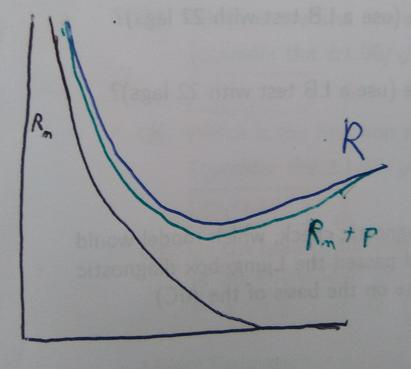
\includegraphics[scale=0.3]{risk_comparison.jpg}
	%\captionsetup{width=13cm}
%\end{figure}

If $g_n$ is the classifier minimizing the penalized empirical risk, then
\begin{equation}
	R_(g_n)\leq \underset{k}{\min}(R(\bar{g}^{(k)})+\text{Penalty}(k))+\text{peanuts},
\end{equation} 
where $\bar{g}^{(k)}=\underset{g\in\mathcal{C}_k}{\text{argmin }}R(g)$.

\section{Machine Learning Algorithms}

\subsubsection{Linear Classifiers}

Suppose that $\Omega= \Re^d$, our data is $\mathcal{D}_n=(X_1,Y_1),\dots,(X_n,Y_n)$, $X_i\in \Omega$, $Y_i\in\{-1,1\}$. We want to learn a linear classifier that has the form of 
\begin{equation}
	g(X)=\text{sign}(w^TX),
\end{equation}
(if $g(X)=0$ then we pick our favorite class). With that, if $d$ is much less than the number of observations the classifier will not overfit. The classification will be done by an hyperplane characterized by its normal vector $w^T$, so we may assume that $\|w\|=1$.\\

Now, the idea is to minimize the risk of our classifier, which means to find the $w^T$ that minimizes the number of mistakes we do. This problem is NP hard when the dimension $d$ is an input. It is doable in time $n^d$ if we fix $d$, but of course this does not solve anything when $d>2$. To tackle the problem we can suppose that the classification is easy, meaning that the data is nearly separable. Then, we have a simple and fast algorithm called \textbf{Perceptron algorithm}.

\subsubsection{Perceptron algorithm}
This algorithm was invented on the 50's and learns a neuron (a linear classifier is basically a neural network with one neuron). \\
Suppose that the data is nearly separable. Let's see the algorithm.\\

1. We start with an arbitrary $w_0$, for example $w_0=0$.\\
2. Then we go through our data points one by one.\\
At time $t$:
\hspace{2cm} if $w_{t-1}X_tY_t> 0$ then we do nothing\\
\hspace{2cm} if $w_{t-1}X_tY_t\leq 0$ then $w_t=w_{t-1}+X_tY_t$.\\
3. Stop when all data points are correctly classified. Cycle through the data the several times if needed. \\
So the linear classifier is $\hat{w}=\su{t}{}X_tY_t\mathbbm{1}_{w_{t-1}X_tY_t\leq 0}$.\\

The beautiful thing is that this algorithm will work, and the time it takes to stop depends on how nice the data is. The niceness of the data is measured by how big is the circle that contains all the points and how far the nearest points to the boundary are (margin). (If the margin is large the algorithm will converge fast).\\

\textbf{Perceptron convergence theorem - Novinkov theorem: }Let $w_*$ be such that $\|w_*\|=1$, $w_*^TX_iY_i>0$ and $\underset{i=1,\dots,n}{\min}|w_*^TX_i|\geq\gamma$ is the margin. Then, the perceptron algorithm holds after at most $\left(\frac{R}{\gamma}\right)^2$ times (adjustments), where $R=\underset{i}{\|X_i\|}$. Observe that it does not depend on the dimension $d$, so if we can guarantee a map in an arbitrary large dimensional space in which we can represent our points that are not too big and can be classified with a large margin, then the perceptron algorithm will work very fast.\\

\textbf{Proof:} Whenever an update is made (noting it as the update number $t^*$), by definition of $w_t$
\begin{equation}
	w_*^Tw_t= w_*^Tw_{t-1} + w_*^TX_tY_t\geq t^*\gamma,	
\end{equation}
because $w_*^TX_tY_t$ is positive and will be always bigger or equal to the margin $\gamma$.
\begin{equation}
	\|w_t\|^2=\|w_{t-1}+X_tY_t\|^2=\|w_{t-1}\|+2w_{t-1}^TX_tY_t+\|X_t\|^2\leq t^*R^2,
\end{equation} 
because $w_{t-1}^TX_tY_t\leq 0$ (we make an update) and $\|X_t\|^2\leq R^2$ (definition of $R$). Now, $\frac{w_*^Tw_t}{\|w_t\|}\geq \frac{t \gamma}{\sqrt{t}R}$ and, since $w_*$ and $\frac{w}{\|w\|}$ are a unit vectors, applying the Cauchy-Schwartz inequality 
\begin{equation}
	1\geq \frac{w_*^Tw_t}{\|w_t\|}\geq \frac{t \gamma}{\sqrt{t}R},
\end{equation} 
so $t\leq\left(\frac{R}{\gamma}\right)^2$ Q.E.D.\\

This result implies that under the conditions that our data is linearly separable in a certain $d$-dimensional space with a margin $\gamma$ and the constrain $R$.

\subsection{Large Margin Classifiers}
 
If the data are not linearly separable, the perceptron algorithm does not halt. In this section, we consider classifiers of the form:
 
\begin{equation*}
	g_f(x)=\begin{cases}
	1, & \text{if} \quad f(x) > 0\\
	-1, & \text{otherwise}.
	\end{cases}
\end{equation*}
where $f:\mathfrak{X} \rightarrow R$.\\
\textbf{Example.} $f(x) = w^TX+c$ for some $w \in \mathbb{R}^d$.
We write $R(f) = R(g_f) = P(-Yf(x)>0) = \mathbb{E}\mathbbm{1}_{-yf(x)>0}$ for the risk or expectation of the number of mislabeled inputs.
 
One usually "convexifies" the optimization problem by replacing the cost function $\mathbbm{1}_x>0$ by a convex (or at least continuous) cost function, such that,
 
$$\phi(x) \geq \mathbbm{1}_x>0$$
 
 
\begin{wrapfigure}{R}{0.4\textwidth}
 	\centering
 	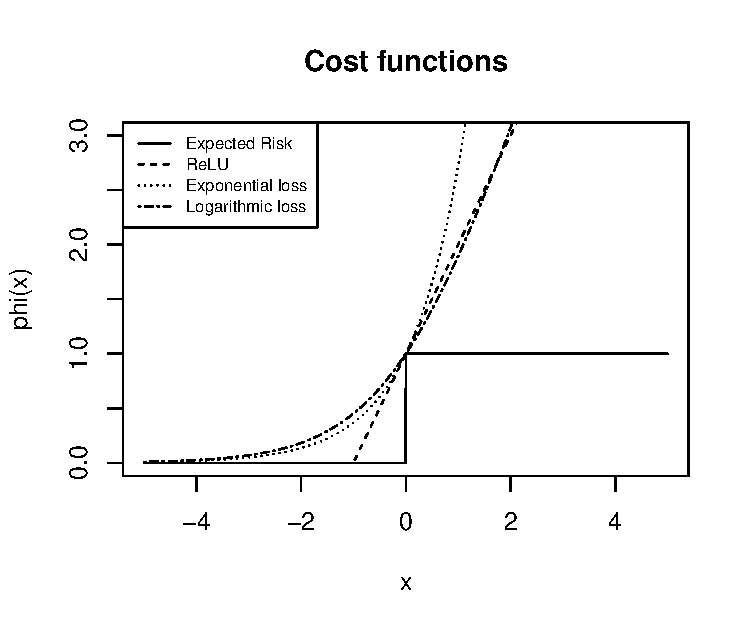
\includegraphics[width=0.45\textwidth]{cost_functions.pdf}
\end{wrapfigure}
 
For instance, in a linear regression setting, $R_n(w) = \frac{1}{n} \sum_{i=1}^{n} \mathbbm{1}_{-yw^Tx_i>0}$, which is not convex, therefore, we need a function $\frac{1}{n} \sum_{i=1}^{n} \phi(-yw^Tx_i>0)$ such that it becomes convex problem, which is easier to optimize.\\
 
\textbf{Example.} ``Hinge loss" a.k.a. Rectified Linear Unit (ReLU)\\
$$\phi(x) = (1+x)_+$$
\textbf{Example.} Exponential loss\\
$$\phi(x) = e^x$$
\textbf{Example.} Logarithmic loss\\
$$\phi(x) = log_2(1+e^x)$$
 
Define $$A(f) = \mathbbm{E}\phi(-yf(x))$$ $$A_n(f) = \frac{1}{n}\sum_i \phi(-yf(x_i)),$$ such that 
$$R(f) \leq A(f)$$
$$R_n(f) \leq A_n(f)$$
 
Suppose $\mathfrak{F}$ is a class of real valued functions and we use data to learn $f_n$ (say, by minimizing $A_n(f)$ over $f \in \mathfrak{F}$). Then,
 
\begin{align*}
	 R(f_n)\leq A(f_n) &\leq A_n(f_n) + \max_{f \in \mathfrak{F}}(A(f) - A_n(f))\\
	 & \approx A_n(f_n) + \mathbbm{E}\ [\max_{f \in \mathfrak{F}}(A(f) - A_n(f))]\\
	 & \leq A_n(f_n) + 2 \mathbbm{E}\ [max |\frac{1}{n} \sum_{i=1}^{n}\sigma \phi(-y_i f(x_i))|]\\
	 & \leq A_n(f) + 2L \mathbbm{E}\ [max |\frac{1}{n} \sum_{i=1}^{n}\sigma f(x_i)|]
\end{align*}
 
\textbf{Example.} $\mathfrak{F} = \{f(x) = w^Tx : ||w|| = 1\}$ then the Rademacher average
 
$$\mathbbm{E} |sup \ \frac{1}{n} \sum \sigma_i w^T x_i| = \mathbbm{E} [sup \ w^T(\frac{1}{n} \sum_{i=1}^{n} \sigma_i x_i)]$$
 
Note that $\sup\limits_{w:||w||=1} \ w^T a = ||a||$, therefore
 
\begin{align*}
	 \mathbbm{E} [sup \ w^T(\frac{1}{n} \sum_{i=1}^{n} \sigma_i x_i)] &=\mathbbm{E} ||\frac{1}{n} \sum_i \sigma_i x_i||\\
	 &\leq \sqrt{\mathbbm{E}||\frac{1}{n} \sum_i \sigma_i x_i||^2}\\
	 &= \sqrt{\mathbbm{E} \sum_j (\frac{1}{n} \sum_i \sigma_i X_i^{(i)})^2}\\
	 &= \frac{1}{n} \sqrt{\mathbbm{E} \sum_i ||X_i||^2}
\end{align*}
 
where $||X_i||^2 \leq R^2$, hence:
 
$$\frac{1}{n} \sqrt{\mathbbm{E} \sum_i ||X_i||^2} \leq \frac{R}{\sqrt{n}}$$
 
which is independent of the dimensions of the problem. If we apply the previous to our inequality $R(f_n) \leq A_n(f) + 2L \mathbbm{E}\ [max |\frac{1}{n} \sum_{i=1}^{n}\sigma f(x_i)|]$, we get
 
$$R(f_n) \leq A_n(f_n) + \frac{2LR}{\sqrt{n}} + c$$
 
where $c$ is a small constant.\\
 
 
\begin{wrapfigure}{L}{0.4\textwidth}
 	\centering
 	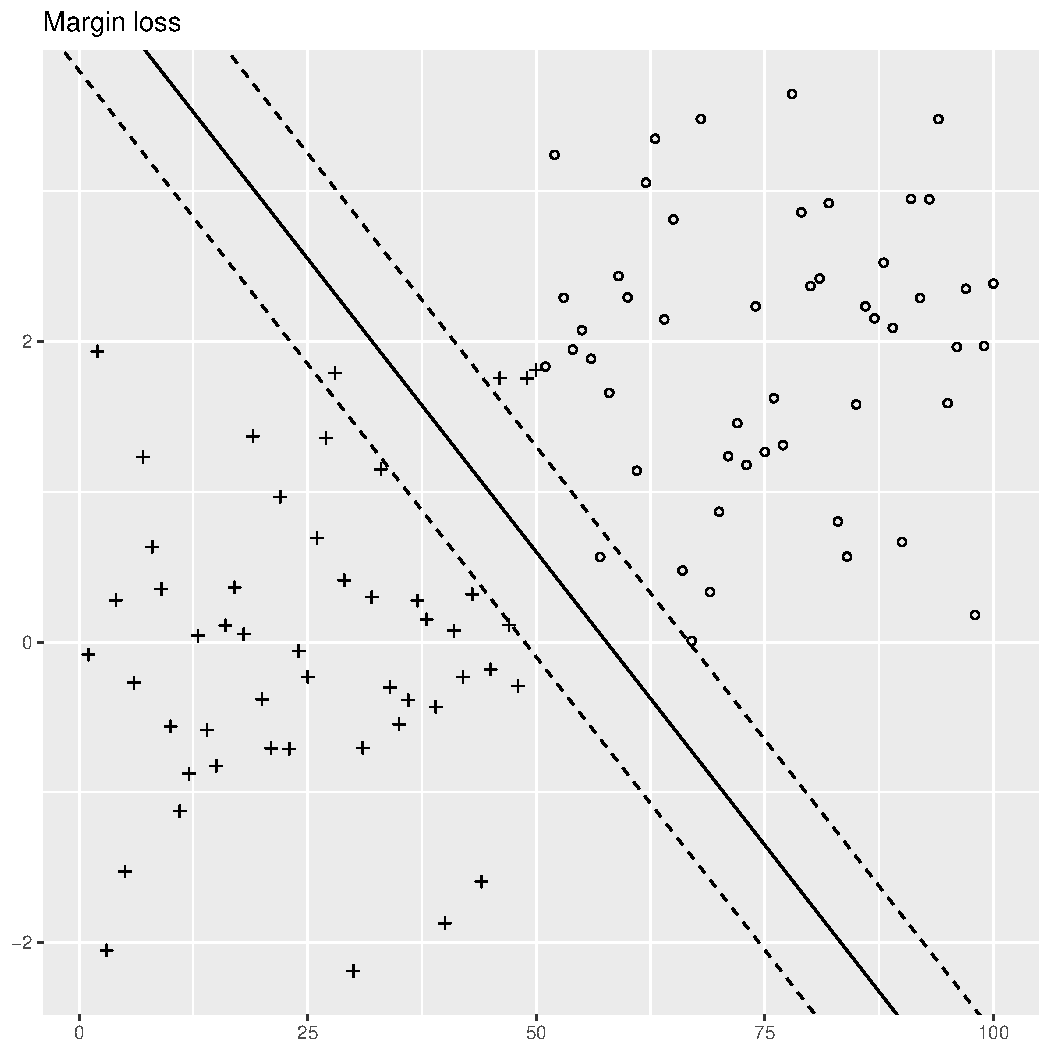
\includegraphics[width=0.35\textwidth]{marginloss.pdf}
 	\caption{\small With the margin loss function, observations within the margins, although correctly classified, add risk as well.}
\end{wrapfigure}
 
Now, consider the "margin loss", then $L = \frac{1}{\gamma}$, and
\begin{align*}
	 R(f_n) &\leq A_n^{\gamma}(f) + \frac{2R}{\gamma\sqrt{n}} + c\\
	 &\leq R_n^{\gamma}(f) + \frac{2R}{\gamma\sqrt{n}} + c
\end{align*}
where the empirical risk $R_n^{\gamma}(f) = \frac{1}{n} \sum_i \mathbbm{1}_{y_iw^Tx_i < -\gamma}$ and $\gamma$ is the distance from our linear classifier that defines a boundary beyond which a correct classification is not considered risk (and viceversa).\\
 
If we manage to classify with a large margin, then $R(f_n)$ will be small no matter the dimension, hence we can map the problem into a larger dimension.
 
Now, consider the ``exponential loss" $\phi(x) = e^x$, then the surrogate risk is $\mathbbm{E}[e^{-yf(x)}] = \mathbbm{E_xE_y}[e^{-y\phi(x)}|X]$, where $\mathbbm{E_y}[e^{-y\phi(x)}|X] = \eta(x) e^{-f(x)} + (1-\eta(x)e^{f(x)})$, and that we can minimize:
 
\begin{align*}
	 arg min &\ \eta e^{-f} + (1-\eta)e^f\\
	 & e^{2f} = \frac{\eta}{1 - \eta}\\
	 & f = \frac{1}{2} ln \frac{\eta}{1 - \eta}
\end{align*}
\linebreak
\linebreak
\\
which is $f^*$ the optimal function. Note that $f^*(x)>0 \Leftrightarrow \eta(x)>\frac{1}{2}$, so $g^* = sgn(f^*(x))$ is the Bayes classifier. The same argument holds for all convex surrogate risks.
 

\section{Kernel methods}

Suppose that $X_i \in R^d$. We may define a ``feature map'' $\Phi : R^d \rightarrow R^D$ where $ D>d$ and work with $(\Phi(X_i), Y_i), \dots, (\Phi(X_n), Y_n)$ and do linear classification in $R^D$. If one achieves a classifier that correctly classifies most of the data with a high margin, then the generalization error is small. The key of kernel methods methods is the inner product $<\Phi(x), \Phi(y)> = \Phi(x)^T \Phi(y) = K(x,y)$.\\

\textbf{Def.} Let $\Omega$ be a vector space (if $x, y \in \Omega$ then $ax + by \in \Omega \ \forall \ a,b \in \mathbb{R})$. An inner product assigns a real number to any $x,y \in \Omega: <x,y>$ such that
\begin{align}
	&<x,y> = <y,x>\\
	&<ax + by, z> = a<x,z> + b<y, z>\\
	&<x,x> = 0 \Leftrightarrow x = 0
\end{align}

\textbf{Example:}\\

$<x,y> = x^Ty \quad \forall ,y \in \mathbb{R}^d$\\

$<x,y> = x^TAy \ \text{if A is symmetric positive definite}$\\

If $\Omega$ is the set of all functions $f: \mathbb{R} \rightarrow \mathbb{R}$ s.t. $\int f(x)^2 dx < \infty$. Then,\\

$<f,g> = \int f(x) g(x) dx$ is an inner product for $f, g \in \Omega$\\

\textbf{Def.} A complete vector space with an inner product is called a Hilbert Space.\\

\textbf{Def.}\ A function $k : \Omega \ \text{x}\ \Omega \rightarrow \mathbb{R}$ is a kernel if there exists a feature map $\Phi : \Omega \rightarrow \mathcal{H}$ such that $k(x,y) = <\Phi(x), \Phi(y)>$.\\

\textbf{Example:} Let $\Omega = \mathbb{R}^2$ and let $\Phi : \mathbb{R}^2 \rightarrow \mathbb{R}^3$ be a feature map defined by

$$
\Phi \begin{bmatrix}
x_1 \\
x_2
\end{bmatrix} = (x^2_1, x^2_2, \sqrt{2}x_1x_2)^T
$$



A linear function in the linear space is:
$$f(x_1,x_2) = ax^2_1 + bx^2_2 + c\sqrt{2}x_1x_2 \quad \text{is a quadratic function in}\ \mathbb{R}^2$$

Then $<\Phi\begin{bmatrix}
x_1 \\
x_2
\end{bmatrix}, \Phi\begin{bmatrix}
y_1 \\
y_2
\end{bmatrix}> = x^2_1y_1^2 + x_2^2y_2^2 + 2x_1x_2y_1y_2 = (x_1y_1 + x_2y_2)^2 = (x^Ty)^2$

Hence, in $\mathbb{R}^2$, $K(x,y) = (x^Ty)^2$ is a kernel function.\\

\textbf{Theorem:} A function $K : \Omega\ \text{x}\ \Omega$ is a kernel if and only if K is a \textbf{positive definite} function, that is, the matrix $(K(x_i,x_j))_{n x n}$ is positive definite $\forall n\ \text{and}\ x_i, \dots, x_n \in \Omega$.

\subsection{Properties of kernels and examples}

If $K_1, K_2$ are kernels on $\Omega$, then 
\begin{itemize}
	\item $K_1 + K_2$, $K_1 \cdot K_2$, $a - K$ are all kernels, for $a>0$.
	\item $K(x,y) = f(x)f(y)$ is a kernel for any $f: \Omega \rightarrow \mathbb{R}$.
	\item $K(x,y) = P(K(x,y))$ is a kernel for any polynomial P with positive coefficients.
	\item $e^{K(x,y)}$ is also a kernel.
	\item $e^{||x-y||^2 /(2\sigma^2)}$ is the Gaussian kernel, where $\sigma$ is any positive number.
	\item $K(x,y) = (x^Ty)^k$ is the polynomial kernel in $\mathbb{R}^d$ for any $k>1$
\end{itemize}

Intuitively, a kernel, being an inner product, is a similarity measure. The inner product $<x,y>$ is higher when the difference between $x,y$ is smaller.

Let's imagine we want to classify news articles. In text classification we have sequences of strings that we need to classify. In these cases one often uses ``string kernels'' as similarity measures. One possibility could be the number of (contiguous) subsequences of a certain length that appear in both strings.

\subsection{Kernel perceptron}

\textbf{Algorithm:}
\begin{enumerate}
	\item[(0)] $w_0 = 0$
	\item[(1)] $w_{t+1} = w_t + X^{t+1}Y^{t+1}$ if $w^T_t X^{t+1}Y^{t+1}<0$. 
\end{enumerate}

That is, we check if our estimate on a new X $w^T_t X^{t+1}$ correctly classifies $Y^{t+1}$. The resulting classifier is

\begin{equation}
g(x) = sgn(w_N^T x) = sgn((\sum_{i=1}^{n} m_i Y_i X_i)^T x) = sgn(\sum_{i=1}^{n}m_i Y_i(X_i^Tx))
\end{equation}

where $m_i$ is the number of times $X_i$ was incorrectly classified.\\

This shows a ``dual'' representation of the algorithm:\\

At time 0, $\alpha_i^{(0)} = 0 \quad \forall \ i = 1, \dots, n$\\
At time t, if $Y^{t+1} \neq sgn(\sum_{i=1}^{n} \alpha_i Y_i X_i^TX^{t+1}) $ then set $\alpha_i^{t+1} = \alpha_i^t + 1$\\

where $\alpha_i$ is the number of times we make a mistake for point $i$.\\ 

Note that $X_i^TX^{t+1}$ can be replaced by $K(X_i, X^{t+1})$ realizing the perceptron algorithm in the Hilbert space in which $K$ is an inner product.


\subsection{Kernelizing regularized risk minimizers}

Suppose we want to compute
\begin{equation}
	\min[f(<w,\Phi(x_1)>, \dots, <w, \Phi (x_n)>+ R(||w||)]
\end{equation}

Where $ R(||w||)$ is a positive increasing penalty. From now on $a_i = <w,\Phi(x_i)>$\\

\textbf{Examples} \\
``Hard-margin'' SVM:
$$f(a_1, \dots, a_n) = \begin{cases}
0\ \text{if}\ Y_i(a_i + b)\geq 1\\
\infty \ \text{otherwise}
\end{cases}$$

In this case, the positive increasing penalty $R(x) = x^2$.\\

That is, we add no risk if we manage to classify with a big margin $b$ but pay infinite if we don't. ``Hard-margin'' SVM only works for data that are linearly separable.\\

``Soft-margin'' SVM:
$$
f(a_1,\dots,a_n) = \frac{1}{n} \sum_{i=1}^{n}(1 - Y_ia_i)_+
$$

In this case, the positive increasing penalty $R(x) = \lambda x^2$\\

Ridge regression:
$$
f(a_1, \dots, a_n) = \frac{1}{n} \sum_{i=1}^{n}(a_i - Y_i)^2
$$

Here again, the regularization parameter $R(x) = \lambda x^2$.\\

LASSO is not of this form because it uses the L1-norm and we need the L2-norm as we will soon see.

\subsection{Representer theorem}

The representer theorem states that the previous minimization problem always has a solution of the form $w = \sum_{i=1}^{n} x_i \Phi(x)$. That is, the representer theorem restricts the search of the solution to a finite dimensional space.

\textbf{Proof.} Let $w^*$ be a solution. We may write $w* = \sum_{i=1}^{n}\alpha_i \Phi(x_i) + u$, where $u$ is orthogonal to the subspace spanned by $\Phi(x_1),\dots, \Phi(x_n)$. So $<u_i, \Phi(x)> = 0 \quad \forall \ i=1,\dots,n$.

\begin{equation}
||w^*||^2 = ||w||^2 + ||u||^2.
\end{equation}


In particular, $||w|| \leq ||w^*||$. Hence $R(||w||) \leq R(||w^*||).$

On the other hand, $<w,\Phi(x_i)> = <w^*, \Phi(x_i)> \ \forall \ i = 1,\dots, n$. Hence, $f(<w,\Phi(x_1)>, \dots, <w, \Phi (x_n)> = f(<w^*,\Phi(x_1)>, \dots, <w^*, \Phi (x_n)>$. So, the minimizer must be in the span of the data $\Phi(x_1), \dots, \Phi(x_n)$. This means that it suffices to search for solutions of the form $w = \sum_{i=1}^{n}\alpha_i \Phi(x_i)$. So,

\begin{equation}
<w,\Phi(x_j)> = \sum_{i=1}^{n} \alpha_i <\Phi(x_i), \Phi(x_j)> = \sum_{i=1}^{n}\alpha_i K(x_i, x_j),
\end{equation}

and

\begin{equation}
||w||^2 = \sum_{i=1}^{n} \sum_{j=1}^{n} \alpha_i \alpha_j <\Phi(x_i), \Phi(x_j)> = \sum_{i=1}^{n}\sum_{j=1}^{n} \alpha_i \alpha_j K(x_i, x_j).
\end{equation}

Therefore, the solution can be computed by the Gram matrix $G = (K(x_i,x_j))_{nxn}$.


\section{Gradient Descend}

 
\end{document}